% ============================================================
% CHAPTER 2: INTRODUCTION
% ============================================================
\chapter{Introduction}

\section{Clinical Background}

\subsection{The Importance of Chest X-ray}

Chest X-ray (CXR) is one of the most common diagnostic imaging methods in medicine:

\begin{itemize}
    \item \textbf{High frequency:} Approximately 2 billion X-ray examinations are performed worldwide annually
    \item \textbf{Low cost:} Much cheaper than CT, MRI
    \item \textbf{Fast results:} Available within minutes
    \item \textbf{Wide application:} Detect pneumonia, tuberculosis, lung cancer, heart diseases
\end{itemize}

\subsection{Challenges in Manual Diagnosis}

\begin{tcolorbox}[colback=red!5!white,colframe=red!75!black,title=Current Problems]
\begin{enumerate}
    \item \textbf{Shortage of radiologists:} Especially in developing countries
    \item \textbf{Heavy workload:} A radiologist may read 100+ images per day
    \item \textbf{Human error:} Fatigue-related misdiagnosis
    \item \textbf{Interpretation variability:} Different doctors may give different diagnoses
\end{enumerate}
\end{tcolorbox}

\section{The Role of Deep Learning}

\subsection{Computer-Aided Diagnosis (CAD)}

Deep Learning opens new possibilities for automating chest X-ray diagnosis:

\begin{tcolorbox}[colback=green!5!white,colframe=green!75!black,title=Benefits of AI in Medical Imaging]
\begin{itemize}
    \item \textbf{Consistency:} Same result for same image
    \item \textbf{Speed:} Analyze images within seconds
    \item \textbf{Scalability:} Can process millions of images
    \item \textbf{Assist radiologists:} As a ``second opinion''
\end{itemize}
\end{tcolorbox}

\subsection{Evolution of Architectures}

\begin{figure}[H]
\centering
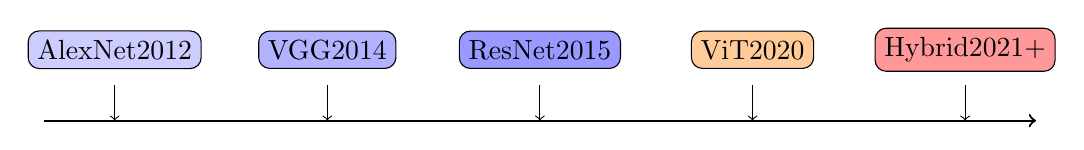
\begin{tikzpicture}[scale=0.9]
    % Timeline
    \draw[->, thick] (0,0) -- (14,0);
    
    % Milestones
    \node[draw, fill=blue!20, rounded corners] at (1,1) {AlexNet\\2012};
    \node[draw, fill=blue!30, rounded corners] at (4,1) {VGG\\2014};
    \node[draw, fill=blue!40, rounded corners] at (7,1) {ResNet\\2015};
    \node[draw, fill=orange!40, rounded corners] at (10,1) {ViT\\2020};
    \node[draw, fill=red!40, rounded corners] at (13,1) {Hybrid\\2021+};
    
    % Arrows
    \draw[->] (1,0.5) -- (1,0);
    \draw[->] (4,0.5) -- (4,0);
    \draw[->] (7,0.5) -- (7,0);
    \draw[->] (10,0.5) -- (10,0);
    \draw[->] (13,0.5) -- (13,0);
\end{tikzpicture}
\caption{Evolution of deep learning architectures for computer vision}
\end{figure}

\section{Research Questions}

The paper addresses the following key questions:

\begin{tcolorbox}[colback=blue!5!white,colframe=blue!75!black,title=Research Questions]
\begin{enumerate}
    \item \textbf{RQ1:} How does CNN baseline perform on chest X-ray classification?
    \item \textbf{RQ2:} Do skip connections in ResNet improve performance?
    \item \textbf{RQ3:} Can Vision Transformer achieve competitive results?
    \item \textbf{RQ4:} Does hybrid ViT-ResNet combine the advantages of both?
\end{enumerate}
\end{tcolorbox}

\section{Paper Contributions}

\paperref{Section 1 - Introduction}

\begin{tcolorbox}[colback=yellow!5!white,colframe=yellow!75!black,title=Paper Quote]
\textit{``In this paper, we present a comparative analysis of a custom CNN, a ResNet-34, and 3 Vision Transformer architectures for multi-classification of chest diseases.''}
\end{tcolorbox}

Main contributions:
\begin{enumerate}
    \item \textbf{Comprehensive comparison:} 5 architectures with the same setup
    \item \textbf{Hybrid ViT-ResNet:} Combining CNN backbone with Transformer
    \item \textbf{Medical imaging application:} Applying ViT to chest X-ray classification
    \item \textbf{Detailed hyperparameter configurations:} For reproducibility
\end{enumerate}

\section{Report Structure}

\begin{table}[H]
\centering
\begin{tabular}{cl}
\toprule
\textbf{Chapter} & \textbf{Content} \\
\midrule
3 & NIH Chest X-ray Dataset \\
4 & CNN: Theory and Code \\
5 & ResNet: Residual Learning \\
6 & Vision Transformer (main chapter) \\
7 & Experiments and Results \\
8 & PyTorch Implementation \\
9 & Conclusion \\
\bottomrule
\end{tabular}
\caption{Report structure}
\end{table}
